\documentclass[12pt]{article}
\usepackage[margin=1in]{geometry}
\usepackage{enumitem}
\usepackage{amsmath}
\usepackage{graphicx}
\usepackage{hyperref}
\usepackage{listings}
\usepackage{xcolor}
\usepackage{tikz}
\usepackage{multirow}
\usetikzlibrary{trees,positioning,arrows,shapes}

% Header and Footer Configuration
\usepackage{fancyhdr}
\usepackage{lastpage}

\setlength{\headheight}{14pt}

\def\myheadertitle{CS 4513 - Database Management: Homework 3 - Problem 3}

\pagestyle{fancy}
\fancyhead{} % clear all header fields
\fancyhead[CO,CE]{\textsc{\myheadertitle}}
\fancyfoot{} % clear all footer fields
\fancyfoot[LO,RE]{\today}
\fancyfoot[RO,LE]{\thepage/\pageref*{LastPage}}
\renewcommand{\headrulewidth}{0.0pt}
\renewcommand{\footrulewidth}{0.0pt}

\begin{document}

\setcounter{tocdepth}{2}
\tableofcontents
\newpage

\section{Problem 3: File Organization and Indexing (GQ3)}

\subsection{Problem Description}

Given the relational database table:

\textbf{VeterinaryClinic (vet\_name, license\_no, clinic\_city, fee\_per\_visit)}

The following insertions are performed on the table VeterinaryClinic:

\begin{enumerate}
    \item Insert record $<$Smith, 12, Tulsa, \$30$>$
    \item Insert record $<$Brown, 45, OKC, \$25$>$
    \item Insert record $<$Wilson, 23, Norman, \$20$>$
    \item Insert record $<$Taylor, 78, OKC, \$25$>$
    \item Insert record $<$Davis, 34, Edmond, \$30$>$
    \item Insert record $<$Clark, 67, Enid, \$35$>$
    \item Insert record $<$Lewis, 89, OKC, \$25$>$
    \item Insert record $<$Walker, 56, Yukon, \$30$>$
    \item Insert record $<$Harris, 90, Tulsa, \$35$>$
\end{enumerate}

\textbf{Assumptions:}
\begin{itemize}
    \item Each block can store up to \textbf{3 veterinarian records}
    \item VeterinaryClinic is organized as a \textbf{sequential file} with \textbf{vet\_name} as the ordering field
\end{itemize}

\subsection{Tasks}

\begin{enumerate}
    \item Show the contents of the file after the last insertion
    \item Show the contents of the dense primary index and secondary index on fee\_per\_visit (assuming index-sequential file)
    \item Show the content of the B+-tree index file on license\_no with order 3
\end{enumerate}

\newpage
\section{Part 1: Sequential File Contents After Last Insertion}

\subsection{Sorted Records by vet\_name}

\small{When organizing as a sequential file ordered by vet\_name, we first sort all records alphabetically:}

\begin{table}[h]
\centering
\begin{tabular}{|c|l|c|l|c|}
\hline
\textbf{Position} & \textbf{vet\_name} & \textbf{license\_no} & \textbf{clinic\_city} & \textbf{fee\_per\_visit} \\
\hline
1 & Brown & 45 & OKC & \$25 \\
2 & Clark & 67 & Enid & \$35 \\
3 & Davis & 34 & Edmond & \$30 \\
4 & Harris & 90 & Tulsa & \$35 \\
5 & Lewis & 89 & OKC & \$25 \\
6 & Smith & 12 & Tulsa & \$30 \\
7 & Taylor & 78 & OKC & \$25 \\
8 & Walker & 56 & Yukon & \$30 \\
9 & Wilson & 23 & Norman & \$20 \\
\hline
\end{tabular}
\caption{Records Sorted by vet\_name}
\end{table}


\subsection{Block Organization (3 records per block)}

{\small
\begin{center}
\fbox{\parbox{0.75\textwidth}{
\small\textbf{BLOCK 0 (Address: 0x000)}\\[0.1cm]
\begin{tabular}{ll}
Record 0 (0x000.0): & $<$Brown, 45, OKC, \$25$>$ \\
Record 1 (0x000.1): & $<$Clark, 67, Enid, \$35$>$ \\
Record 2 (0x000.2): & $<$Davis, 34, Edmond, \$30$>$ \\
\end{tabular}
}}
\end{center}

\vspace{0.2cm}

\begin{center}
\fbox{\parbox{0.75\textwidth}{
\small\textbf{BLOCK 1 (Address: 0x001)}\\[0.1cm]
\begin{tabular}{ll}
Record 0 (0x001.0): & $<$Harris, 90, Tulsa, \$35$>$ \\
Record 1 (0x001.1): & $<$Lewis, 89, OKC, \$25$>$ \\
Record 2 (0x001.2): & $<$Smith, 12, Tulsa, \$30$>$ \\
\end{tabular}
}}
\end{center}

\vspace{0.2cm}

\begin{center}
\fbox{\parbox{0.75\textwidth}{
\small\textbf{BLOCK 2 (Address: 0x002)}\\[0.1cm]
\begin{tabular}{ll}
Record 0 (0x002.0): & $<$Taylor, 78, OKC, \$25$>$ \\
Record 1 (0x002.1): & $<$Walker, 56, Yukon, \$30$>$ \\
Record 2 (0x002.2): & $<$Wilson, 23, Norman, \$20$>$ \\
\end{tabular}
}}
\end{center}
}

\newpage

\subsection{Detailed Address Mapping}

\begin{table}[h]
\centering
\begin{tabular}{|c|c|c|l|}
\hline
\textbf{Record Address} & \textbf{Block} & \textbf{Position} & \textbf{Data} \\
\hline
0x000.0 & Block 0 & Pos 0 & $<$Brown, 45, OKC, \$25$>$ \\
0x000.1 & Block 0 & Pos 1 & $<$Clark, 67, Enid, \$35$>$ \\
0x000.2 & Block 0 & Pos 2 & $<$Davis, 34, Edmond, \$30$>$ \\
\hline
0x001.0 & Block 1 & Pos 0 & $<$Harris, 90, Tulsa, \$35$>$ \\
0x001.1 & Block 1 & Pos 1 & $<$Lewis, 89, OKC, \$25$>$ \\
0x001.2 & Block 1 & Pos 2 & $<$Smith, 12, Tulsa, \$30$>$ \\
\hline
0x002.0 & Block 2 & Pos 0 & $<$Taylor, 78, OKC, \$25$>$ \\
0x002.1 & Block 2 & Pos 1 & $<$Walker, 56, Yukon, \$30$>$ \\
0x002.2 & Block 2 & Pos 2 & $<$Wilson, 23, Norman, \$20$>$ \\
\hline
\end{tabular}
\caption{Complete Address Mapping}
\end{table}

\newpage
\section{Part 2: Index-Sequential File with Indexes}

\subsection{Dense Primary Index on vet\_name}

A \textbf{dense primary index} has one index entry for \textbf{every search key value} in the data file.

\begin{table}[h]
\centering
\begin{tabular}{|l|c|}
\hline
\textbf{Search Key (vet\_name)} & \textbf{Record Pointer (Address)} \\
\hline
Brown & 0x000.0 \\
Clark & 0x000.1 \\
Davis & 0x000.2 \\
Harris & 0x001.0 \\
Lewis & 0x001.1 \\
Smith & 0x001.2 \\
Taylor & 0x002.0 \\
Walker & 0x002.1 \\
Wilson & 0x002.2 \\
\hline
\end{tabular}
\caption{Dense Primary Index on vet\_name}
\end{table}

\textbf{Explanation:}
\begin{itemize}
    \item Each veterinarian name has an entry pointing to its exact record location
    \item Total entries: 9 (one for each record)
    \item This is a \textbf{primary index} because vet\_name is the ordering field
    \item This is \textbf{dense} because every search key value has an index entry
\end{itemize}

\newpage

\subsection{Secondary Index on fee\_per\_visit}

A \textbf{secondary index} is built on a non-ordering field. For fee\_per\_visit, multiple records may have the same value, so we use a structure with record lists.

\begin{table}[h]
\centering
\begin{tabular}{|c|p{6cm}|}
\hline
\textbf{Search Key} & \textbf{Record Pointers (Addresses)} \\
\textbf{(fee\_per\_visit)} & \\
\hline
\$20 & 0x002.2 (Wilson) \\
\hline
\multirow{3}{*}{\$25} & 0x000.0 (Brown) \\
 & 0x001.1 (Lewis) \\
 & 0x002.0 (Taylor) \\
\hline
\multirow{3}{*}{\$30} & 0x000.2 (Davis) \\
 & 0x001.2 (Smith) \\
 & 0x002.1 (Walker) \\
\hline
\multirow{2}{*}{\$35} & 0x000.1 (Clark) \\
 & 0x001.0 (Harris) \\
\hline
\end{tabular}
\caption{Secondary Index on fee\_per\_visit}
\end{table}

\textbf{Explanation:}
\begin{itemize}
    \item This is a \textbf{secondary index} because fee\_per\_visit is NOT the ordering field
    \item Each unique fee value points to ALL records with that fee
    \item The index is sorted by fee\_per\_visit for efficient searching
    \item Total unique entries: 4 (\$20, \$25, \$30, \$35)
\end{itemize}

\newpage
\section{Part 3: B+-Tree Index on license\_no (Order 3)}

\subsection{B+-Tree Properties}

For a B+-tree of \textbf{order n = 3}:

\begin{itemize}
    \item \textbf{Maximum keys per node:} n - 1 = 2 keys
    \item \textbf{Minimum keys per internal node:} $\lceil n/2 \rceil$ - 1 = $\lceil 1.5 \rceil$ - 1 = 1 key
    \item \textbf{Minimum keys per leaf node:} $\lceil n/2 \rceil$ - 1 = 1 key
    \item \textbf{Maximum children per internal node:} n = 3
    \item \textbf{Minimum children per internal node:} $\lceil n/2 \rceil$ = 2
\end{itemize}

\subsection{License Numbers in Sorted Order}

The license numbers in sorted order are: 12, 23, 34, 45, 56, 67, 78, 89, 90

\subsection{Step-by-Step B+-Tree Construction}

\subsubsection{Insertions 1-2: Insert 12, 23}

After inserting 12 and 23:
\begin{center}
\fbox{[12, 23]}
\end{center}

\subsubsection{Insertion 3: Insert 34 (causes split)}

Node becomes [12, 23, 34] which exceeds maximum of 2 keys. Split and promote middle key (23):

\begin{center}
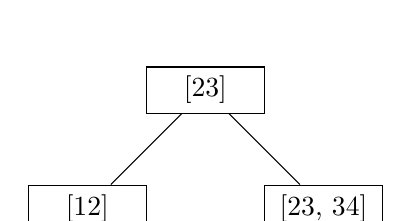
\begin{tikzpicture}[level distance=1.5cm,
  level 1/.style={sibling distance=3cm},
  every node/.style={rectangle,draw,minimum width=1.5cm}]
  \node {[23]}
    child {node {[12]}}
    child {node {[23, 34]}};
\end{tikzpicture}
\end{center}

\subsubsection{Insertion 4: Insert 45 (causes split)}

Leaf [23, 34] becomes [23, 34, 45]. Split and promote 34:

\begin{center}
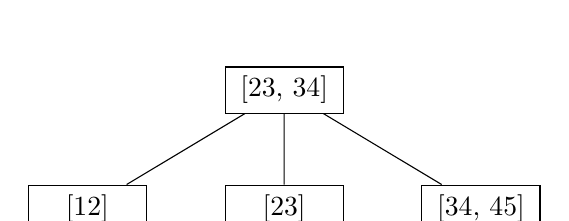
\begin{tikzpicture}[level distance=1.5cm,
  level 1/.style={sibling distance=2.5cm},
  every node/.style={rectangle,draw,minimum width=1.5cm}]
  \node {[23, 34]}
    child {node {[12]}}
    child {node {[23]}}
    child {node {[34, 45]}};
\end{tikzpicture}
\end{center}

\subsubsection{Insertion 5: Insert 56 (causes split and root split)}

Leaf [34, 45] becomes [34, 45, 56]. Split and promote 45. Root [23, 34] becomes [23, 34, 45], which is full. Split root:

\begin{center}
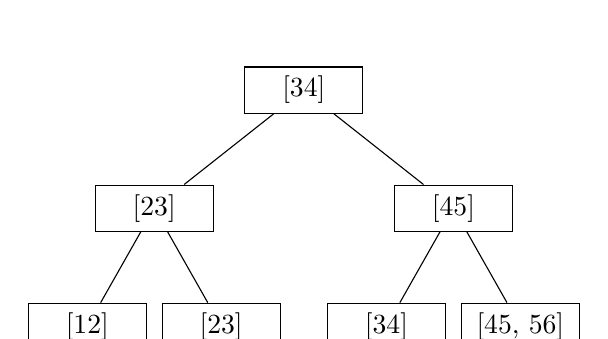
\begin{tikzpicture}[level distance=1.5cm,
  level 1/.style={sibling distance=3.8cm},
  level 2/.style={sibling distance=1.7cm},
  every node/.style={rectangle,draw,minimum width=1.5cm}]
  \node {[34]}
    child {node {[23]}
      child {node {[12]}}
      child {node {[23]}}
    }
    child {node {[45]}
      child {node {[34]}}
      child {node {[45, 56]}}
    };
\end{tikzpicture}
\end{center}

\subsubsection{Insertion 6: Insert 67 (causes split)}

Leaf [45, 56] becomes [45, 56, 67]. Split and promote 56:

\begin{center}
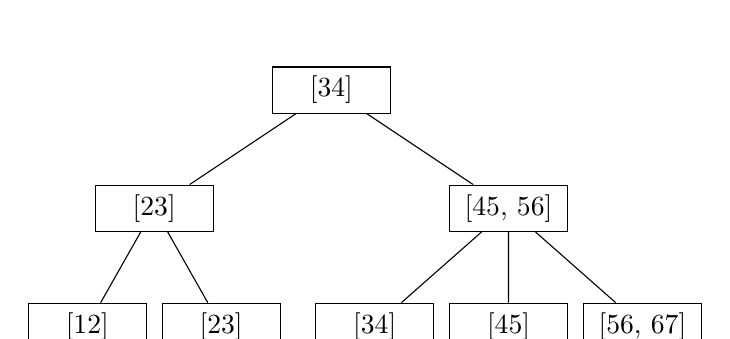
\begin{tikzpicture}[level distance=1.5cm,
  level 1/.style={sibling distance=4.5cm},
  level 2/.style={sibling distance=1.7cm},
  every node/.style={rectangle,draw,minimum width=1.5cm}]
  \node {[34]}
    child {node {[23]}
      child {node {[12]}}
      child {node {[23]}}
    }
    child {node {[45, 56]}
      child {node {[34]}}
      child {node {[45]}}
      child {node {[56, 67]}}
    };
\end{tikzpicture}
\end{center}

\subsubsection{Insertion 7: Insert 78 (causes split)}

Leaf [56, 67] becomes [56, 67, 78]. Split and promote 67:

\begin{center}
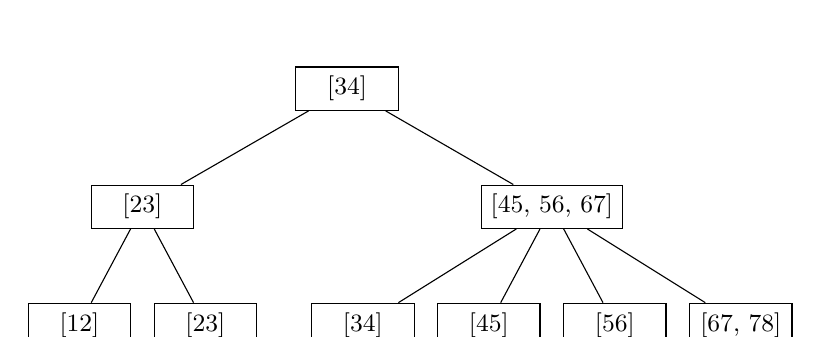
\begin{tikzpicture}[level distance=1.5cm,
  level 1/.style={sibling distance=5.2cm},
  level 2/.style={sibling distance=1.6cm},
  every node/.style={rectangle,draw,minimum width=1.3cm,font=\small}]
  \node {[34]}
    child {node {[23]}
      child {node {[12]}}
      child {node {[23]}}
    }
    child {node {[45, 56, 67]}
      child {node {[34]}}
      child {node {[45]}}
      child {node {[56]}}
      child {node {[67, 78]}}
    };
\end{tikzpicture}
\end{center}

Internal node [45, 56, 67] has 3 keys (exceeds max of 2). Split and promote 56 to root:

\begin{center}
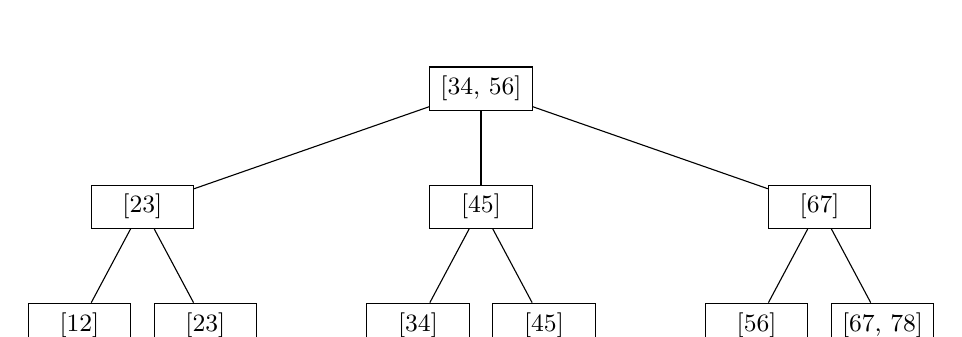
\begin{tikzpicture}[level distance=1.5cm,
  level 1/.style={sibling distance=4.3cm},
  level 2/.style={sibling distance=1.6cm},
  every node/.style={rectangle,draw,minimum width=1.3cm,font=\small}]
  \node {[34, 56]}
    child {node {[23]}
      child {node {[12]}}
      child {node {[23]}}
    }
    child {node {[45]}
      child {node {[34]}}
      child {node {[45]}}
    }
    child {node {[67]}
      child {node {[56]}}
      child {node {[67, 78]}}
    };
\end{tikzpicture}
\end{center}

\subsubsection{Insertion 8: Insert 89 (causes split)}

Leaf [67, 78] becomes [67, 78, 89]. Split and promote 78:

\begin{center}
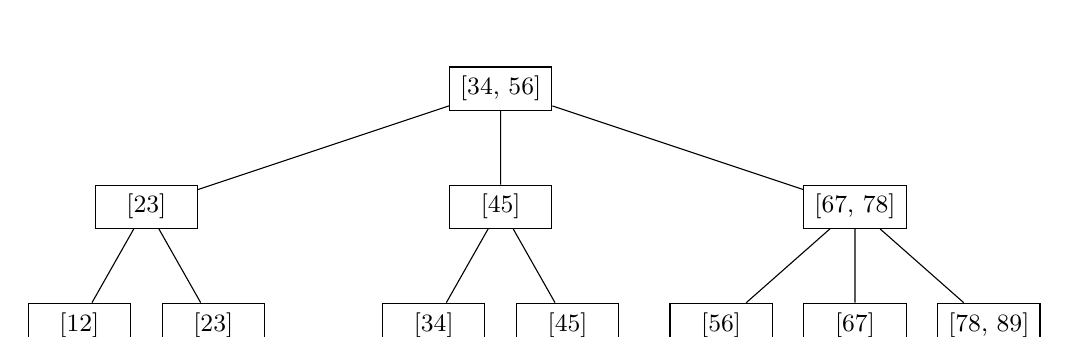
\begin{tikzpicture}[level distance=1.5cm,
  level 1/.style={sibling distance=4.5cm},
  level 2/.style={sibling distance=1.7cm},
  every node/.style={rectangle,draw,minimum width=1.3cm,font=\small}]
  \node {[34, 56]}
    child {node {[23]}
      child {node {[12]}}
      child {node {[23]}}
    }
    child {node {[45]}
      child {node {[34]}}
      child {node {[45]}}
    }
    child {node {[67, 78]}
      child {node {[56]}}
      child {node {[67]}}
      child {node {[78, 89]}}
    };
\end{tikzpicture}
\end{center}

\subsubsection{Insertion 9: Insert 90 (causes split and root split)}

Leaf [78, 89] becomes [78, 89, 90]. Split and promote 89. Internal node [67, 78] becomes [67, 78, 89], which exceeds max. Split and promote 78 to root. Root [34, 56] becomes [34, 56, 78], exceeds max. Split root and promote 56:

\subsection{Final B+-Tree Structure}

\begin{figure}[h]
\centering
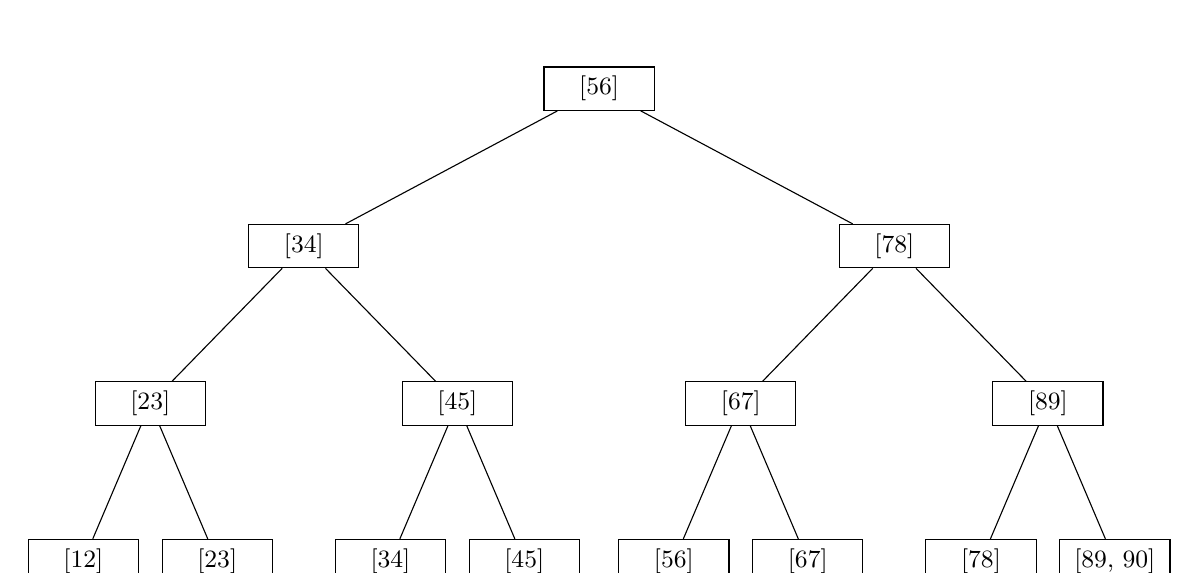
\begin{tikzpicture}[
  level distance=2cm,
  level 1/.style={sibling distance=7.5cm},
  level 2/.style={sibling distance=3.9cm},
  level 3/.style={sibling distance=1.7cm},
  every node/.style={rectangle,draw,minimum width=1.4cm,align=center,font=\small}]
  
  \node {[56]}
    child {node {[34]}
      child {node {[23]}
        child {node {[12]}}
        child {node {[23]}}
      }
      child {node {[45]}
        child {node {[34]}}
        child {node {[45]}}
      }
    }
    child {node {[78]}
      child {node {[67]}
        child {node {[56]}}
        child {node {[67]}}
      }
      child {node {[89]}
        child {node {[78]}}
        child {node {[89, 90]}}
      }
    };
\end{tikzpicture}
\caption{Final B+-Tree on license\_no}
\end{figure}

\newpage

\subsection{Leaf Node Contents with Data Pointers}

The leaf nodes contain the following license numbers with pointers to the actual veterinarian records:

\begin{table}[h]
\centering
\begin{tabular}{|c|l|c|}
\hline
\textbf{License No} & \textbf{vet\_name} & \textbf{Leaf Node} \\
\hline
12 & Smith & [12] \\
23 & Wilson & [23] \\
34 & Davis & [34] \\
45 & Brown & [45] \\
56 & Walker & [56] \\
67 & Clark & [67] \\
78 & Taylor & [78] \\
89 & Lewis & [89, 90] \\
90 & Harris & [89, 90] \\
\hline
\end{tabular}
\caption{Leaf Node to Data Record Mapping}
\end{table}

\textbf{Note:} In a B+-tree, leaf nodes are typically linked horizontally (not shown in diagram) to support efficient range queries.

\subsection{B+-Tree Properties Verification}

\begin{itemize}
    \item \textbf{Root has between 2 and 3 children:} Root [56] has 2 children - Yes
    \item \textbf{Internal nodes have between 2 and 3 children:} All internal nodes have 2 children - Yes
    \item \textbf{All leaves are at the same level:} Yes, depth = 3 - Correct
    \item \textbf{Leaf nodes have between 1 and 2 keys:} All leaves comply - Yes
    \item \textbf{Keys are in ascending order:} Yes - Correct
    \item \textbf{No duplicate license\_no:} Correct (unique constraint) - Yes
\end{itemize}

\newpage
\section{Summary}

This solution demonstrates three file organization and indexing methods for the VeterinaryClinic database:

\begin{itemize}
    \item \textbf{Part 1:} Sequential file organization with 9 records sorted by vet\_name and stored in 3 blocks (3 records per block)
    
    \item \textbf{Part 2:} Index-sequential file with:
    \begin{itemize}
        \item Dense primary index on vet\_name (9 entries)
        \item Secondary index on fee\_per\_visit (4 unique fee values: \$20, \$25, \$30, \$35)
    \end{itemize}
    
    \item \textbf{Part 3:} B+-tree of order 3 on license\_no with final structure having root [56], demonstrating step-by-step insertion and splits
\end{itemize}

\vspace{0.5cm}

All three approaches provide different trade-offs between storage overhead, search efficiency, and maintenance complexity, with sequential files being simplest, index-sequential adding fast lookup capability, and B+-trees offering the best performance for dynamic data with frequent updates.

\end{document}

